\documentclass[12pt]{extarticle}

\usepackage{amsmath}
\usepackage{unicode-math}
\usepackage{xltxtra}
\usepackage{xgreek}

\setmainfont{Liberation Serif}

\usepackage{tabularx}

\pagestyle{empty}

\usepackage{geometry}
 \geometry{a4paper, total={190mm,275mm}, left=10mm, top=10mm}

 \usepackage{graphicx}
 \graphicspath{ {images/} }

 \usepackage{wrapfig}

\begin{document}

\begin{table}
    \small
    \begin{tabularx}{\textwidth}{ c X r }
        \begin{tabular}{ c }
            
\includegraphics[scale=0.4]{ελληνική}          \\
            ΕΛΛΗΝΙΚΗ ΔΗΜΟΚΡΑΤΙΑ                            \\
            ΥΠΟΥΡΓΕΙΟ ΠΑΙΔΕΙΑΣ \& ΘΡΗΣΚΕΥΜΑΤΩΝ             \\
            ΠΕΡΙΦΕΡΕΙΑΚΗ Δ/ΝΣΗ Α/ΘΜΙΑΣ \& Β/ΘΜΙΑΣ  ΕΚΠ/ΣΗΣ \\
            ΚΕΝΤΡΙΚΗΣ ΜΑΚΕΔΟΝΙΑΣ                           \\
            Δ/ΝΣΗ Β/ΘΜΙΑΣ ΕΚΠ/ΣΗΣ ΑΝ. ΘΕΣ/ΝΙΚΗΣ            \\
            10ο ΓΕΝΙΚΟ ΛΥΚΕΙΟ ΘΕΣ/ΝΙΚΗΣ
        \end{tabular}
         &  &
        \begin{tabular}{ r }
            Σχολικό Έτος: 2022 - 2023     \\
            Εξ. Περίοδος: Μαΐου - Ιουνίου \\
            Μάθημα: Μαθηματικά Γ Λυκείου  \\
            Εισηγητής: Λόλας              \\ \\
            Θεσσαλονίκη, 25 / 05 / 2023
        \end{tabular}
    \end{tabularx}
\end{table}

\part*{\centering{Θέματα}}
\section*{Θέμα 1}
\noindent
\begin{enumerate}
    \item[α)] Να αποδείξετε ότι αν $Α$ ένα ενδεχόμενο ενός δειγματοχώρου και $Α'$ το συμπλήρωμά του, τότε $$P(Α')=1-P(Α)$$. \hspace*{\fill} \textbf{Μονάδες 10}
    \item[β)] Έστω δύο ενδεχόμενα $Α$ και $Β$ και η πρόταση
        "το ενδεχόμενο $Γ$ ορίζεται ως το ενδεχόμενο να συμβείτο $Α$ και να μην συμβεί $Β$"

        \begin{enumerate}
            \item[i.] Να γράψετε το ενδεχόμενο $Γ$ ως πράξη συνόλων μεταξύ των $Α$ και $Β$
            \item[ii.] Να σχηματίσετε διάγραμμα Venn όπου θα φαίνονται ταυτόχρονα τα ενδεχόμενα $Α$, $Β$ και $Γ$
        \end{enumerate}\hspace*{\fill} \textbf{Μονάδες 3 + 2}

    \item[γ)] Να χαρακτηρίσετε τις παρακάτω προτάσεις με Σωστό ή Λάθος
        \begin{enumerate}
            \item [i.] Η μέση τιμή είναι μέτρο θέσης.
            \item [ii.] Ο χρόνος είναι ποιοτική μεταβλητή.
            \item [iii.] Για κάθε ενδεχόμενο $Α$ ισχύει $P(Α)>0$.
            \item [iv.] Αν $CV < 0.1$ τότε τα δεδομένα είναι ομοιογενή.
            \item [v.] Η διάμεσος είναι η μέση τιμή.\hspace*{\fill} \textbf{Μονάδες 10}
        \end{enumerate}

\end{enumerate}

\section*{Θέμα 2 (36753)}
\noindent

Ρωτήθηκαν 120 φοιτητές και φοιτήτριες και 120 μαθητές και μαθήτριες της Γ΄ λυκείου, πού προτιμούν να πάνε διακοπές το καλοκαίρι, μεταξύ βουνού και θάλασσας. Όλοι και όλες έδωσαν μία από τις δύο απαντήσεις αυτές. Τα αποτελέσματα των απαντήσεών τους φαίνονται στο παρακάτω στοιβαγμένο ραβδόγραμμα, αλλά από τη ράβδο «Μαθητές/τριες Γ΄ λυκείου» λείπει το μέρος που αντιστοιχεί στην απάντηση «θάλασσα».

\begin{figure}[h]
    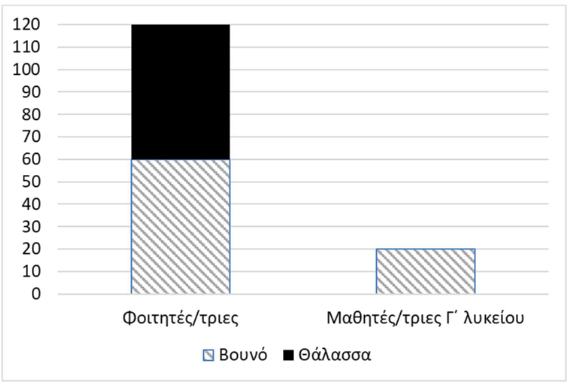
\includegraphics[width=0.5\textwidth]{2023.png}
    \centering
\end{figure}

\begin{enumerate}
    \item[α)]
        \begin{enumerate}
            \item[i.] Πόσοι/ες μαθητές/τριες Γ΄ λυκείου απάντησαν ότι προτιμούν βουνό;\hspace*{\fill} \textbf{Μονάδες 5}
            \item[ii.] Να υπολογίσετε πόσοι/ες μαθητές/τριες Γ΄ λυκείου απάντησαν ότι προτιμούν θάλασσα.\hspace*{\fill} \textbf{Μονάδες 6}
        \end{enumerate}
    \item[β)] Να χαρακτηρίσετε ως σωστή (Σ) ή λανθασμένη (Λ) την παρακάτω πρόταση.

        «Οι περισσότεροι/ες από τους φοιτητές/τριες απάντησαν ότι προτιμούν βουνό.»
        \hspace*{\fill} \textbf{Μονάδες 5}
    \item[γ)] Να μεταφέρετε στην κόλλα σας και να συμπληρώσετε το παραπάνω στοιβαγμένο ραβδόγραμμα.

        \hspace*{\fill} \textbf{Μονάδες 9}
\end{enumerate}

\section*{Θέμα 3}
\noindent

Οι βαθμοί στα 4 μαθήματα Πανελλαδικών είναι $18$, $15$, $17$, $10$. Να βρείτε
\begin{enumerate}
    \item[α)] την μέγιστη και την ελάχιστη βαθμολογία \hspace*{\fill} \textbf{Μονάδες 4}
    \item[β)] το εύρος \hspace*{\fill} \textbf{Μονάδες 4}
    \item[γ)] την διάμεσο \hspace*{\fill} \textbf{Μονάδες 4}
    \item[δ)] την μέση τιμή \hspace*{\fill} \textbf{Μονάδες 4}
    \item[ε)] την διακύμανση \hspace*{\fill} \textbf{Μονάδες 5}
    \item[στ)] την τυπική απόκλιση \hspace*{\fill} \textbf{Μονάδες 4}
\end{enumerate}
Δίνεται $\sqrt{9.5}=3,08$

\section*{Θέμα 4 (32738)}
\noindent

Ένα κουτί περιέχει 2 κόκκινες γραβάτες και 3 πράσινες γραβάτες, από τις οποίες ο Γιώργος για κάθε μέρα από τις επόμενες πέντε μέρες, θα παίρνει τυχαία μία γραβάτα να φορέσει.
\begin{enumerate}
    \item[α)] Για το παραπάνω πείραμα τύχης να γράψετε τον δειγματικό χώρο $Ω$, όπου το αποτέλεσμα ΠΚΚΠΚ για παράδειγμα, σημαίνει ότι την πρώτη, την τέταρτη και την πέμπτη μέρα ο Γιώργος θα φορέσει πράσινη γραβάτα, ενώ τη δεύτερη και την τρίτη μέρα θα φορέσει κόκκινη γραβάτα. \hspace*{\fill} \textbf{Μονάδες 7}
    \item[β)] Να βρείτε τις πιθανότητες των ενδεχομένων, ο Γιώργος:
        \begin{enumerate}
            \item[i.] να φορέσει πράσινη γραβάτα την πρώτη μέρα,
            \item[ii.] να μη φορέσει πράσινη γραβάτα την πρώτη μέρα,
            \item[iii.] να φορέσει κάθε μέρα, διαφορετικό χρώμα γραβάτας από την προηγούμενη μέρα.
        \end{enumerate} \hspace*{\fill} \textbf{Μονάδες 18}
\end{enumerate}
\begin{table}[htb]
    \begin{tabularx}{\textwidth}{ X c X c X}
         &
        \begin{tabular}[t]{ c }
            Ο Δ/ντης \\ \\ \\ \\
            Παπαδημητρίου Χρήστος
        \end{tabular}
         &   &
        \begin{tabular}[t]{ c }
            Ο εισηγητής \\ \\ \\ \\
            Λόλας Κωνσταντίνος
        \end{tabular}
         &
    \end{tabularx}
\end{table}
\end{document}
